\documentclass[dvipdfmx,journal]{IEEEtran}

\usepackage{algorithm}      % \begin{algorithm}
\usepackage{algorithmic}    % \begin{algorithmic}
\usepackage{amsmath}        % \begin{align*}
\usepackage{amssymb}        % \mathbb{A}
\usepackage{amsthm}         % \newtheorem
\usepackage{ascmac}         % \begin{screen}
\usepackage{bm,bbm}         % \bm{A}, \bbm{1}
\usepackage{booktabs}       % \toprule, \midrule, \bottomrule
\usepackage{caption}        % \captionsetup
\usepackage{enumitem}       % \begin{enumerate}[label=(\alph*)]
\usepackage{geometry}       % \geometry{margin=1in}
\usepackage{hyperref}       % \href{URL}{text}
\usepackage{ifthen}         % \ifthenelse
\usepackage{lipsum}         % \lipsum
\usepackage{mathrsfs}       % \mathscr{A}
\usepackage{mathtools}      % \mathrlap
\usepackage{optidef}        % \begin{mini*}{x}{f(x)}{}{}
\usepackage{orcidlink}      % \orcidlink
\usepackage{physics}        % \qty, \norm, \abs
\usepackage{subfiles}       % \subfile{file}
\usepackage{thm-restate}    % \begin{restatable}{theorem}{thm}
\usepackage{tikz}           % \begin{tikzpicture}
\usepackage{xparse}         % \NewDocumentCommand
% \usepackage{calc}         % \setlength
% \usepackage{cancel}       % \cancel
% \usepackage{parskip}      % \setlength{\parskip}{0.5em}
% \usepackage{csvsimple}    % \csvautotabular
% \usepackage{diagbox}      % \diagbox
% \usepackage{dsfont}       % \mathds{1}
% \usepackage{epsfig}       % \epsfig
% \usepackage{fancybx}      % \ovalbox
% \usepackage{float}        % \begin{figure}[H]
% \usepackage{lipsum}       % \lipsum
% \usepackage{listings}     % \begin{lstlisting}
% \usepackage{makecell}     % \makecell{L1\L2}
% \usepackage{multicol}     % \begin{multicols}{2}
% \usepackage{multirow}     % \multirow
% \usepackage{nicematrix}   % \begin{NiceMatrix}
% \usepackage{qcircuit}     % \Qcircuit
% \usepackage{siunitx}      % \SI{1}{\second}
% \usepackage{stfloats}     % \begin{figure*}
% \usepackage{subcaption}   % \begin{subfigure}
% \usepackage{ulem}         % \sout
% \usepackage[hyphens]{url} % \url
% \usepackage{wrapfig}      % \begin{wrapfigure}
% \usepackage[all]{xy}      % \xymatrix
% \usepackage[dvipdfmx]{graphicx}
% \usepackage[square, sort, comma, numbers]{natbib}

\geometry{margin=1in}
\hypersetup{colorlinks=true,linkcolor=blue,citecolor=blue,urlcolor=blue}

\definecolor{cA}{HTML}{0072BD}
\definecolor{cB}{HTML}{EDB120}
\definecolor{cC}{HTML}{77AC30}
\definecolor{cD}{HTML}{D95319}

\newcommand{\red}[1]{\textcolor{red}{#1}}
\newcommand{\blue}[1]{\textcolor{blue}{#1}}
\newcommand{\cyan}[1]{\textcolor{cyan}{#1}}
\newcommand{\gray}[1]{\textcolor{gray}{#1}}
\newcommand{\green}[1]{\textcolor{green}{#1}}
\newcommand{\brown}[1]{\textcolor{brown}{#1}}
\newcommand{\black}[1]{\textcolor{black}{#1}}
\newcommand{\st}{\text{ s.t. }}
\newcommand{\Img}[1]{\mathrm{Im}\qty(#1)}
\newcommand{\Ker}[1]{\mathrm{Ker}\qty(#1)}
\newcommand{\Supp}[1]{\mathrm{supp}\qty(#1)}
\newcommand{\Rank}[1]{\mathrm{rank}\qty(#1)}
\newcommand{\floor}[1]{\left\lfloor #1 \right\rfloor}
\newcommand{\ceil}[1]{\left\lceil #1 \right\rceil}
% C++ (https://tex.stackexchange.com/questions/4302/prettiest-way-to-typeset-c-cplusplus)
\newcommand{\Cpp}{C\nolinebreak[4]\hspace{-.05em}\raisebox{.4ex}{\relsize{-3}{\textbf{++}}}}
% https://tex.stackexchange.com/questions/28836/typesetting-the-define-equals-symbol
\newcommand{\defeq}{\coloneqq}
\newcommand{\eqdef}{\eqqcolon}
% https://tex.stackexchange.com/questions/5502/how-to-get-a-mid-binary-relation-that-grows
\newcommand{\relmiddle}[1]{\mathrel{}\middle#1\mathrel{}}
\newcommand{\Lhopital}{L'H\^optial}

\DeclareMathOperator{\Proj}{Proj}
\DeclareMathOperator{\Exp}{Exp}
\DeclareMathOperator{\Hess}{Hess}
\DeclareMathOperator{\Retr}{Retr}
\DeclareMathOperator{\Span}{span}
% \DeclareMathOperator{\myGrad}{grad}
% \renewcommand{\grad}{\myGrad}

% https://tex.stackexchange.com/questions/564216/newcommand-for-each-letter
\ExplSyntaxOn
\NewDocumentCommand{\definealphabet}{mmmm}{
\int_step_inline:nnn{`#3}{`#4}{
\cs_new_protected:cpx{#1 \char_generate:nn{##1}{11}}{
\exp_not:N #2{\char_generate:nn{##1}{11}}}}}
\ExplSyntaxOff

\definealphabet{bb}{\mathbb}{A}{Z}
\definealphabet{rm}{\mathrm}{A}{Z}
\definealphabet{cal}{\mathcal}{A}{Z}
\definealphabet{frak}{\mathfrak}{a}{z}
% \definealphabet{scr}{\mathscr}{A}{Z}
% \definealphabet{frak}{\mathfrak}{A}{Z}

\newtheorem{theorem}{Theorem}
\newtheorem{proposition}{Proposition}
\newtheorem{lemma}{Lemma}
\newtheorem{definition}{Definition}
\newtheorem{corollary}{Corollary}
\newtheorem{remark}{Remark}
\newtheorem{example}{Example}
\newtheorem{assumption}{Assumption}

% https://qiita.com/rityo_masu/items/efd44bc8f9229e014237
\allowdisplaybreaks[4]

% \lstset{
%   language=Python,numbers=left,frame=single,breaklines=true,lineskip=-0.9ex,xleftmargin=3zw,xrightmargin=0zw,
%   basicstyle=\ttfamily,ndkeywordstyle=\small,identifierstyle=\small,numberstyle=\scriptsize,
%   commentstyle=\color[rgb]{0,0.6,0},stringstyle=\small\ttfamily\color[rgb]{0.89,0.55,0},keywordstyle=\small\bfseries\color[rgb]{0.28,0.28,0.95},
% }

\usetikzlibrary{
  3d,
  % fit,
  calc,
  math,
  matrix,
  patterns,
  backgrounds,
  arrows.meta,
  shapes.geometric,
  % decorations.pathmorphing,
}

% \graphicspath{{./fig/}}

% \providecommand{\main}{.}
\newboolean{isMain}
\setboolean{isMain}{true}

\begin{document}

\title{Fruchterman--Reingold Algorithm with Random Subspace Newton}
\author{Hiroki Hamaguchi\,\orcidlink{0009-0005-7348-1356}}
\date{\today}
\maketitle

\begin{abstract}
  The abstract goes here.
  \lipsum[1]
\end{abstract}

\begin{IEEEkeywords}
  Graph drawing, Fruchterman--Reingold algorithm, Random Subspace method.
\end{IEEEkeywords}

\section{Introduction}

% グラフ自動描画法とその応用
% https://www.jstage.jst.go.jp/article/jssst/12/4/12_4_335/_article/-char/ja

\IEEEPARstart{G}{raph} is a mathematical structure representing pairwise relationships between objects, and graph drawing is one of the most fundamental tasks in data science. Indeed, Numerous general algorithms have been proposed for graph drawing~\cite{tutteHowDrawGraph1963,chrobakLineartimeAlgorithmDrawing1995,sugiyamaMethodsVisualUnderstanding1981,ghassemitoosiSimulatedAnnealingPreProcessing2016}
Among these, one of the most popular strategies is force-directed algorithms.

In force-directed algorithms, the graph is modeled as a physical system of particles. These include methods such as the Kamada--Kawai (KK) layout~\cite{kamadaAlgorithmDrawingGeneral1989} using shortest path distances for a cost function, and the Fruchterman--Reingold (FR) layout~\cite{fruchtermanGraphDrawingForcedirected1991}, which is the primary focus of this paper.

The FR algorithm is one of the most widely used force-directed algorithms. It is also implemented in many modern graph drawing libraries such as NetworkX~\cite{osti_960616}, Graphviz~\cite{ellsonGraphvizOpenSource2002}, and igraph~\cite{csardiIgraphSoftwarePackage2006}. The FR layout is based on a physical model of a system of particles and springs, and FR algorithm seeks the equilibrium of the forces between nodes.

However, since both the KK layout and the FR layout requires to compute the forces or energies between all pairs of vertices, they have a high computational cost of $\order{n^2}$ per iteration, where $n$ is the number of vertices in the graph. To address this kind of computational burden, several methods have been proposed. One strategy is to approximate the $n$-body simulation using hierarchical methods such as the fast multipole method~\cite{greengardFastAlgorithmParticle1987}, the Barnes--Hut approximation~\cite{barnesHierarchicalLogForcecalculation1986}, multilevel approaches~\cite{Hu2006EfficientHF}, or stress majorization~\cite{gansnerGraphDrawingStress2005}.

Another approach is to accelerate the optimization algorithm directly, which aligns with the spirit of our work. Recent researches have accelerated the algorithms for FR layout and KK layout through various methods, including GPU parallel architectures~\cite{gajdosParallelFruchtermanReingold2016}, numerical optimization techniques such as L-BFGS~\cite{6183577}, and Stochastic Gradient Descent (SGD)~\cite{8419285}.

Based on such advances, in this paper, we investigate the ability of another algorithm: Random Subspace Newton (RSN). The RSN method is a variant of the Newton method that uses a random subspace to approximate the Hessian matrix. The RSN method and its variant have been proposed in the context of optimization problems~\cite{NEURIPS2019_bc6dc48b,fujiRandomizedSubspaceRegularized2022,cartisRandomisedSubspaceMethods2022,higuchiFastConvergenceSecondOrder2024}.

The rest of the paper is organized as follows.
In Section~\ref{sec:preliminary}, we define the optimization problem for the FR algorithm.
In Section~\ref{sec:RSN}, we introduce the Random Subspace method and report a its problem when directly applied to the FR algorithm.
In Section~\ref{sec:algorithm}, we propose a new algorithm that combines the FR algorithm with the Random Subspace method.
In Section~\ref{sec:experiment}, we present the experimental results.
Finally, we conclude and discuss future work in Section~\ref{sec:discussion}.

\begin{figure}[t]
  \begin{minipage}{0.49\hsize}
    \centering
    \includegraphics[width=\columnwidth]{/home/hari64boli64/University/FruchtermanReingoldByRandomSubspace/doc/jagmesh1_FR_50iter.png}
  \end{minipage}
  \begin{minipage}{0.49\hsize}
    \centering
    \includegraphics[width=\columnwidth]{/home/hari64boli64/University/FruchtermanReingoldByRandomSubspace/doc/jagmesh1_LBFGS_50iter.png}
  \end{minipage}
  \caption{Comparison of the FR algorithm (left, NetworkX) and L-BFGS-B (right, my implementation) on the \texttt{jagmesh1} dataset.}
\end{figure}

\section{Preliminary}\label{sec:preliminary}

\begin{figure*}[t]
  \begin{minipage}{0.49\hsize}
    \centering
    \begin{tikzpicture}
      \def\d{4}
      \def\r{0.3}
      \def\u{1.0}
      \coordinate (M1) at (0,0);
      \coordinate (M2) at (\d,0);

      \draw (M1) circle(\r) node {$v_i$};
      \draw (M2) circle(\r) node {$v_j$};

      \draw (0,+1.6*\r) -- (0,+2.4*\r);
      \draw (\d,+1.6*\r) -- (\d,+2.4*\r);
      \draw[{Latex[length=4,width=3]}-{Latex[length=4,width=3]}] ($(M1)+(90:2*\r)$) -- ($(M2)+(90:2*\r)$)
      node[midway,circle,fill=white,inner sep=0] {$d$};

      \draw[->,thick,line cap=round] (+\r,0) -- (+\u,0) node[right] {$F^a_{i,j}(d)$};
      \draw[->,thick,line cap=round] (-\r,0) -- (-\u,0) node[left] {$F^r(d)$};

      \draw[dashed,domain=3.9:-3.1,samples=1000,smooth,variable=\x] plot(\x,{-0.7+(pow((\d-\x)/\d,3)/3-ln((\d-\x)/\d))/2.2});
      \node [star,
        minimum size=0.25cm,
        star point ratio=2.25,
        inner sep=0pt,
        draw, fill=black]
      at (0,{-0.7+(1/3)/2.2}) {};

      \node at (-2.7,0.4) {$E_{i,j}(d)$};
    \end{tikzpicture}
    \caption{
    Fruchterman--Reingold model.
    The equilibrium of the attractive force $F^a_{i,j}(d)$ and the repulsive force $F^r(d)$ is the optimal distance $d=k/\sqrt[3]{a_{i,j}}$.
    }
  \end{minipage}
  \begin{minipage}{0.49\hsize}
    \centering
    \includegraphics[width=\columnwidth]{energy_3d.png}
    \caption{Energy function $E_{i,j}(d)$ for $a_{i,j} = 1$ and $k = 1$. Although $E_{i,j}$ is convex for $d$, but not for $x_i$.}
    \label{fig:label}
  \end{minipage}
\end{figure*}

In this section, we define an optimization problem for FR algorithm.
Let $\bbR_{> 0}$ be a set of positive real numbers,
and $A = (a_{i,j}) \in \bbR_{> 0}^{n \times n}$ be an adjacency matrix of a graph $G = (V, E)$.
FR algorithm is also applicable to a directed unconnected graph, but we focus on the undirected connected graph for simplicity. In particular, the connectivity of the graph is indispensable for the solution to be bounded, and for a unconnected graph, we can apply algorithms to each connected component independently, if necessary.

Each vertex $v_i \in V$ is assigned a position $x_i \in \bbR^d$ and we define $x = (x_1, \dots, x_n) \in \bbR^{d \times n}$ as a matrix of positions.
For an parameter $k$ and a distance $d$ between two vertices $v_i$ and $v_j$, Fruchterman and Reingold~\cite{fruchtermanGraphDrawingForcedirected1991} defined the power of attraction $F_{i,j}^a: \bbR_{> 0} \to \bbR$ and the power of repulsion $F^r: \bbR_{> 0} \to \bbR$ as
\begin{equation*}
  F_{i,j}^a(d) \defeq \frac{a_{i,j} d^2}{k}, \quad F^r(d) \defeq -\frac{k^2}{d}.
\end{equation*}
The total energy for these powers $E_{i,j} : \bbR_{> 0} \to \bbR$, stress of the graph, is defined as
\begin{align*}
  E_{i,j}(d) & \defeq \int_{0}^{d} F_{i,j}^a(r) \dd{r} + \int_{\infty}^{d} F^r(r) \dd{r} \\
             & = \frac{a_{i,j} d^3}{3k} - k^2\log{d}.
\end{align*}

The energy function $E_{i,j}$ is convex for $a_{i,j} \in \bbR_{> 0}$ and minimized when $d = k/\sqrt[3]{a_{i,j}}$, but is not Lipschitz continuous.
Based on these energies, the optimization problem for FR algorithm is defined as
\begin{mini}
  {x \in \bbR^{d \times n}}
  {f(x) \defeq \sum_{i<j} E_{i,j}(d_{i,j})}
  {\label{eq:fr}}
  {}
\end{mini}
where $d_{i,j} = \norm{x_i - x_j}$ is the Euclidean distance.

As pointed out in~\cite{tunkelang1999numerical},
the FR algorithm is a gradient descent method for the energy function $f$, with constant step size and cooling schedule.

\section{Random Subspace Newton} \label{sec:RSN}

In this section, we introduce the Random Subspace Newton (RSN) method and report a its problem when directly applied to the FR algorithm.

\subsection{What is Random Subspace Newton}

First, we introduce the RSN method.
RSN is a variant of the Newton's method.
For $N$ variables problem, the Newton's method requires to compute the Hessian matrix of size $N \times N$ at each iteration, which poses a high computational cost for large-scale problems.
One way to address this issue is to employ quasi-Newton methods, such as the L-BFGS method, which approximates the Hessian directly, and has also been applied in graph drawing~\cite{6183577}.
In contrast, RSN focuses on a subspace of dimension $S$ randomly selected from the solution space and utilizes the exact Hessian matrix of size $S \times S$ defined on this subspace.
Since $S \ll N$, the computational cost per iteration is significantly reduced.

The RSN method resembles the stochastic coordinate descent method, which updates only a subset of the variables at each iteration using gradient information. The difference is that RSN uses the Hessian matrix to determine the update direction, bringing the method closer to the Newton method.

Moreover, recent studies have explored its application not only to convex optimization problems but also to non-convex optimization problems~\cite{fujiRandomizedSubspaceRegularized2022}.

\subsection{Random Subspace Newton for FR Algorithm}

we define a function $f_i: \bbR^{d} \to \bbR$ for $1 \leq i \leq n$ as
\begin{equation*}
  f_i(x_i) \defeq \sum_{j \neq i} E_{i,j}(d_{i,j}).
\end{equation*}
The gradient and the Hessian of $f_i$ are
\begin{gather*}
  \nabla f_i(x_i) = \sum_{j \neq i} \qty(\frac{a_{i,j}d_{i,j}}{k} - \frac{k^2}{d_{i,j}^2}) (x_i-x_j), \\
  \nabla^2 f_i(x_i) = \sum_{j \neq i} \qty(\frac{a_{i,j}d_{i,j}}{k} - \frac{k^2}{d_{i,j}^2}) I_d +      \\
  \sum_{j \neq i} \qty(\frac{a_{i,j}}{k d_{i,j}} + \frac{2k^2}{d_{i,j}^4}) (x_i - x_j)(x_i - x_j)^\top.
\end{gather*}

In this way, the problem exhibits a natural affinity with the RSN method, as it inherently defines a subspace of the solution space for the FR layout.

Moreover, the effectiveness of Stochastic Gradient Descent (SGD) for KK layout is well-documented in~\cite{8419285}.
In contrast to the KK layout, where each function is individually determined by $\frac{k_{i,j}}{2}(d_{i,j}-l_{i,j})^2$ based on the actual distance between vertices $d_{i,j}$ and their optimal distance $l_{i,j}$, the FR layout assigns the same value, $-k^2\log{d_{i,j}}$, to all pairs of points without direct edges, making SGD relatively less effective for the FR layout.

However, the report in the KK layout, which highlights that optimization focusing on each edge yields favorable results, suggests that optimization focusing on each vertex, such as methods utilizing RSN, may also be effective in the FR layout.

In this situation, our research aims to investigate the effectiveness of the RSN method for the FR layout.

\subsection{problem of RSN for FR Algorithm}

\begin{figure*}[t]
  \centering
  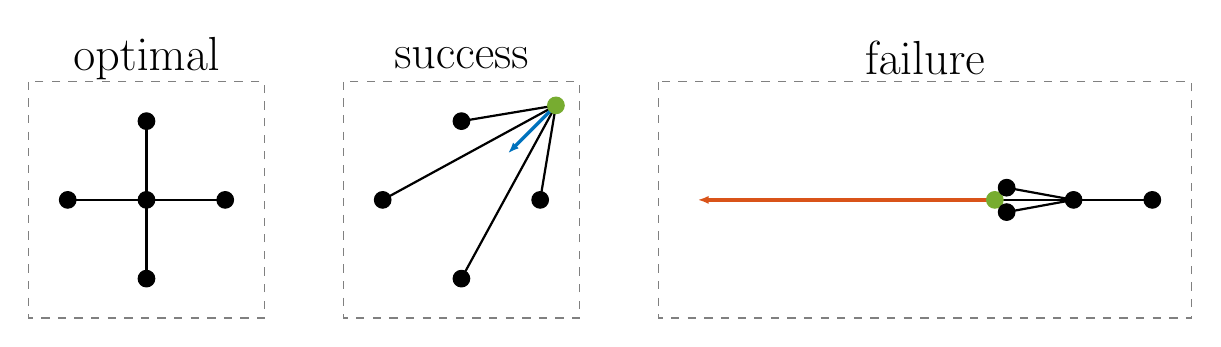
\begin{tikzpicture}
    \foreach \xA/\yA/\xB/\yB/\xC/\yC/\xD/\yD/\xE/\yE/\arrowX/\arrowY/\xShift/\xRect/\arrowV/\caZero/\caOne/\desc in {
        0/0/-1/0/0/1/0/-1/1/0/0/0/0/-1.5/a0/black/black/optimal,
        1.2/1.2/-1/0/0/1/0/-1/1/0/0.592271758813887/0.592271758813887/4/-1.5/a0/cC/black/success,
        0/0/-1/0/-0.85/0.155/-0.85/-0.155/1/0/-4.77422/0/11.77422/-5.27422/a1/black/cC/failure}{
        \begin{scope}[xshift=\xShift cm]
          \draw[dashed,color=gray,line width=0.5pt] (\xRect, 1.5) rectangle (1.5, -1.5);
          \node at ({(\xRect+1.5)/2}, 1.8) {\LARGE{\desc}};
          \coordinate (a0) at (\xA, \yA);
          \coordinate (a1) at (\xB, \yB);
          \coordinate (a2) at (\xC, \yC);
          \coordinate (a3) at (\xD, \yD);
          \coordinate (a4) at (\xE, \yE);
          \draw[thick] (a0) -- (a1);
          \draw[thick] (a0) -- (a2);
          \draw[thick] (a0) -- (a3);
          \draw[thick] (a0) -- (a4);

          \ifthenelse{\equal{\arrowX}{0} \AND \equal{\arrowY}{0}}{}{
          \ifthenelse{\equal{\desc}{success}}{
          \draw[-{Latex[length=4,width=3]},very thick,cA] (\arrowV) -- (\arrowX, \arrowY);
          }{
          \draw[-{Latex[length=4,width=3]},very thick,cD] (\arrowV) -- (\arrowX, \arrowY);
          }}

          \filldraw[draw=\caZero,fill=\caZero] (a0) circle (3pt);
          \filldraw[draw=\caOne,fill=\caOne]   (a1) circle (3pt);
          \filldraw[draw=black,fill=black] (a2) circle (3pt);
          \filldraw[draw=black,fill=black] (a3) circle (3pt);
          \filldraw[draw=black,fill=black] (a4) circle (3pt);
        \end{scope}
      }
  \end{tikzpicture}
  \caption{
    Visualization of the problem of the subspace method.
    Let a graph as shown in the left (optimal), where $k$ and all positive edge weights $a_{i,j}$ are set to 1.
    For the situation in the middle (success), the RSN works effectively.
    However, in the situation depicted on the right (failure),
    where the points are set as $x_0=(0,0), x_1=(-1,0), x_2=(-0.85,0.155), x_3=(-0.85,-0.155), x_4=(1,0)$,
    the Hessian for the subspace of $x_1$ is approximately
    $
      \begin{pmatrix} 1.841 & 0 \\ 0 & 1.159 \end{pmatrix}
    $.
    This Hessian, while positive definite and not ill-conditioned, leads to a Newton direction that clearly deviates significantly from the global optimal solution.
  }
  \label{fig:why_RSN_failed}
\end{figure*}

However, unfortunately, the RSN method is not necessarily effective for the FR layout.
As shown in Figure \ref{fig:why_RSN_failed}, although the energy function \( f_i \) with respect to the position \( x_i \) of each vertex is convex in the FR layout, the overall energy function \( f \) with respect to \( x_i \) is not convex.

\section{Algorithm} \label{sec:algorithm}


\section{Experiment} \label{sec:experiment}

We used dataset from \cite{davis2011university} and MatrixMarket \cite{boisvertMatrixMarketWeb1997}.

\url{https://reference.wolfram.com/language/tutorial/GraphDrawingIntroduction.html}

\section{Discussion} \label{sec:discussion}

In this paper, we investigated the effectiveness of the Random Subspace Newton method for the Fruchterman--Reingold algorithm.

\subsection{Combination with Other Methods}



\subsection{Application to Other Problems}



\section{Acknowledgment}

The author would like to express our sincere gratitude to PL Poirion and Andi Han for their insightful discussions, which have greatly inspired and influenced this research.

\ifthenelse{\boolean{isMain}}{
  \bibliographystyle{IEEEtran}
  \bibliography{FruchtermanReingoldByRandomSubspace}
}{}

\appendices

\section{Optimal Scaling}

When we optimize a placement for FR-layout with an initial placement obtained, for instance through KK-layout, scaling the initial placement at first can often yield better results than directly using the unmodified initial placement.
In this section, we address the problem of finding the optimal scaling factor that minimizes the energy function for a given configuration.

\subsection{Optimal Scaling Algorithm}

Formulating the optimization through scaling, the task reduces to selecting an appropriate scaling factor $x \in \bbR_{> 0}$ that minimizes the following energy function:

\begin{align*}
  \phi(x) \defeq {} & \qty(\sum_{i < j} \frac{w_{ij} (xd_{ij})^3}{3k}) - k^2 \sum_{i < j} \log(x d_{ij})                                  \\
  \begin{split}
    = {} & x^3 \qty(\sum_{i < j} \frac{w_{ij} d_{ij}^3}{3k}) - \log(x)(k^2 n(n-1))\\
    & - k^2 \sum_{i < j} \log(d_{ij})
  \end{split} \\
  \phi'(x) = {}     & 3x^2 \qty(\sum_{i < j} \frac{w_{ij} d_{ij}^3}{3k}) - \frac{k^2 n(n-1)}{x}                                           \\
  \phi''(x) = {}    & 6x \qty(\sum_{i < j} \frac{w_{ij} d_{ij}^3}{3k}) + \frac{k^2 n(n-1)}{x^2}
\end{align*}

The function $\phi(x)$ is convex, and we can find the optimal scaling factor $x$ by using Newton's method.

This algorithm achieves sufficient convergence within a few iterations, and when we pre-compute the coefficients of $\phi(x)$ with $w_{i,j} > 0$, the time complexity is just $\order{\abs{E}}$.

\section{Another approach based on the Hexagonal Lattice}

todo

\end{document}